% THIS IS SIGPROC-SP.TEX - VERSION 3.1
% WORKS WITH V3.2SP OF ACM_PROC_ARTICLE-SP.CLS
% APRIL 2009
%
% It is an example file showing how to use the 'acm_proc_article-sp.cls' V3.2SP
% LaTeX2e document class file for Conference Proceedings submissions.
% ----------------------------------------------------------------------------------------------------------------
% This .tex file (and associated .cls V3.2SP) *DOES NOT* produce:
%       1) The Permission Statement
%       2) The Conference (location) Info information
%       3) The Copyright Line with ACM data
%       4) Page numbering
% ---------------------------------------------------------------------------------------------------------------
% It is an example which *does* use the .bib file (from which the .bbl file
% is produced).
% REMEMBER HOWEVER: After having produced the .bbl file,
% and prior to final submission,
% you need to 'insert'  your .bbl file into your source .tex file so as to provide
% ONE 'self-contained' source file.
%
% Questions regarding SIGS should be sent to
% Adrienne Griscti ---> griscti@acm.org
%
% Questions/suggestions regarding the guidelines, .tex and .cls files, etc. to
% Gerald Murray ---> murray@hq.acm.org
%
% For tracking purposes - this is V3.1SP - APRIL 2009

\documentclass{acm_proc_article-sp}

\begin{document}

\title{Prioritizing ThreadSanitizer race reports with large or input-controlled vulnerable windows}
%
% You need the command \numberofauthors to handle the 'placement
% and alignment' of the authors beneath the title.
%
% For aesthetic reasons, we recommend 'three authors at a time'
% i.e. three 'name/affiliation blocks' be placed beneath the title.
%
% NOTE: You are NOT restricted in how many 'rows' of
% "name/affiliations" may appear. We just ask that you restrict
% the number of 'columns' to three.
%
% Because of the available 'opening page real-estate'
% we ask you to refrain from putting more than six authors
% (two rows with three columns) beneath the article title.
% More than six makes the first-page appear very cluttered indeed.
%
% Use the \alignauthor commands to handle the names
% and affiliations for an 'aesthetic maximum' of six authors.
% Add names, affiliations, addresses for
% the seventh etc. author(s) as the argument for the
% \additionalauthors command.
% These 'additional authors' will be output/set for you
% without further effort on your part as the last section in
% the body of your article BEFORE References or any Appendices.

\numberofauthors{2} %  in this sample file, there are a *total*
% of EIGHT authors. SIX appear on the 'first-page' (for formatting
% reasons) and the remaining two appear in the \additionalauthors section.
%
\author{
% You can go ahead and credit any number of authors here,
% e.g. one 'row of three' or two rows (consisting of one row of three
% and a second row of one, two or three).
%
% The command \alignauthor (no curly braces needed) should
% precede each author name, affiliation/snail-mail address and
% e-mail address. Additionally, tag each line of
% affiliation/address with \affaddr, and tag the
% e-mail address with \email.
%
% 1st. author
\alignauthor
Mateus Braga\\
	\affaddr{Columbia University}\\
       \email{mateus.a.braga@gmail.com}
% 2nd. author
\alignauthor
Jintack Lim\\
	\affaddr{Columbia Univeristy}\\
       \email{jintack@cs.columbia.edu}
}

% There's nothing stopping you putting the seventh, eighth, etc.
% author on the opening page (as the 'third row') but we ask,
% for aesthetic reasons that you place these 'additional authors'
% in the \additional authors block, viz.
% Just remember to make sure that the TOTAL number of authors
% is the number that will appear on the first page PLUS the
% number that will appear in the \additionalauthors section.

\maketitle
\begin{abstract}
This paper provides a sample of a \LaTeX\ document which conforms to
the formatting guidelines for ACM SIG Proceedings.
It complements the document \textit{Author's Guide to Preparing
ACM SIG Proceedings Using \LaTeX$2_\epsilon$\ and Bib\TeX}. This
source file has been written with the intention of being
compiled under \LaTeX$2_\epsilon$\ and BibTeX.

The developers have tried to include every imaginable sort
of ``bells and whistles", such as a subtitle, footnotes on
title, subtitle and authors, as well as in the text, and
every optional component (e.g. Acknowledgments, Additional
Authors, Appendices), not to mention examples of
equations, theorems, tables and figures.

To make best use of this sample document, run it through \LaTeX\
and BibTeX, and compare this source code with the printed
output produced by the dvi file.
\end{abstract}

% A category with the (minimum) three required fields
\category{H.4}{Information Systems Applications}{Miscellaneous}
%A category including the fourth, optional field follows...
\category{D.2.8}{Software Engineering}{Metrics}[complexity measures, performance measures]

\terms{Theory}

\keywords{ACM proceedings, \LaTeX, text tagging} % NOT required for Proceedings

\section{Introduction}

\subsection{Motivation}
The motivation of our work comes from the real world need to specify bug severity and priority. The tools developed in this project can help developers find out how exploitable a concurrency bug is by giving them information of how large the vulnerability window is, or can be [Cite Junfeng]. With this information, a developer can better prioritize the concurrency bugs found.


\subsection{Vulnerability Window}
A vulnerability window is the interval between two memory accesses to the same location that should be atomic but it is not. We say that two accesses are atomic if they are never interleaved by another thread's access in a unserializable way. The AVIO paper [Cite AVIO paper] describes which interleavings are serializable and which are not.

Every concurrent application defines code regions that are expected to be atomic. The programmers are responsible for enforcing the isolation of these code regions from any unserializable interleavings by means of synchronization (i.e. locks, barriers, semaphores, and transactions). A failure to enforce this isolation is called a concurrency bug and creates a vulnerability window. A vulnerability window can be exploited by an attacker to cause the program to deviate from its correct behavior, and the bigger its size, the easier for the attacker to successfully exploit the bug. In this project we are only concerned with the size of the vulnerability window. A further study on the possible ways to break the security of the application by means of a vulnerability window is left for future work.

\section{Degisn}
\subsection{Proposal}
The goal of this project is to add information about the vulnerability window to a ThreadSanitizer data race report. This information can then help developers find out the severity of each data race by informing how large the vulnerability window is, or can be. We propose a modified version of ThreadSanitizer and some tools that partially achieves this goal. We understand that there are many ways to improve our tools and we consider this project a first step toward successfully accomplishing the goal.

\subsection{ThreadSanitizer and Data Races}
ThreadSanitizer is a fast open-source happens-before data race detector developed by Google [Cite ThreadSanitizer]. It performs dynamic analysis and reports data races in C/C++ and Go applications. An application has a data race when two of its threads performs unsynchronized accesses to the same memory location. Because of its happens-before approach, no false positive is reported [Cite ThreadSanitizer], so every reported race is real or a bug in the tool. ThreadSanitizer's execution time overhead is 2-20x, and its memory usage overhead is 5-10x. This overhead is considered acceptable for many applications, and that is why ThreadSanitizer has been used by many projects inside and outside Google (i.e. Chromium, Firefox).

According to C++ standard, C standard, POSIX, Go memory model and other standards, any data race is undefined behavior [Cite Intel benign race]. This means that a compiler can assume that accesses without synchronization can be subject to optimizations that could result in code that does not faithfully represents the source code. This also means that code that contains data races can behavior differently from one compiler to another. There are many resources that explains why there is no benign data races in these languages [Cite …], so fixing all data races is recommended. 

One interesting aspect of a data race bug is that it does not need to cause the application to deviate from correct behavior to be detected. This is great because data race bugs can be one of the hardest bugs to reproduce, since it depends on a bug-triggering execution interleaving to be exposed. ThreadSanitizer, for example, detects data races by keeping track of the happens-before relationships between accesses to every memory location. It knows when the application has a data race if it sees two accesses to the same location without any happens-before relationship. This can be detected even when both accesses are performed far away from each other. While this is great when we want to find them, this aspect makes it hard for us to find the vulnerability window associated with a data race reported.

The following image is an example of a ThreadSanitizer data race report. A report always contains the follow information: the current and previous accesses that are not synchronized, their operation, source-code location, size, memory location, thread and what mutexes were held at the time of each access.

\begin{figure}
\centering
\epsfig{file=images/tsan_output.eps, width=\linewidth,}
\caption{ThreadSanitizer output}
\end{figure}

\subsection{Approaches}
In order to associate the vulnerability window information to each race report, we need to first find the vulnerability window associated with the report. For this step, we sticked to the idea suggested by Professor Junfeng of using the next access to the racy location by each of the reported threads. To achieve this, we tried two different approaches: 
Perform static analysis to find the next access after the racy locations reported:
	In this approach we search for another access to the same racy location reported nearby the racy instruction using LLVM's Alias Analysis.
	Modifying ThreadSanitizer to provide the next access location in each thread:
		In this approach we modify ThreadSanitizer to give us the position of the next access to the racy location previously reported in each of the threads in the report.

		After identifying the vulnerability window associated with each report, the next step is to measure how large this window is, or can be. In order to do this, we tried two different approaches:
		Doing dynamic data flow analysis to find input-controlled variables that could increase the size of the vulnerability window:
		In this approach we use LLVM's DataFlowSanitizer to keep track of which memory locations are influenced by input and uses this information to reason about how the vulnerability window can be made larger.
		Further modifying ThreadSanitizer to provide dynamic vulnerability window information:
			In this approach we modify ThreadSanitizer to give us information like total amount of memory allocated and time of report to later use it to determine how large the window is.

\section{Implementations}
\subsection{Static Alias Analysis}
Our first implementation attempt was to go through all the LLVM instructions in the functions that contains the racy accesses and use the closest memory instruction whose pointer operand alias with the the racy location to form the window. Our intuition was that the alias analysis would know what other load/store instruction was also pointing to the racy location when focusing on just one function. 

We also tried using the Memory Dependence analysis, which promises to be able to answer the question of what preceding memory operations a given instruction depends on, either at an intra- or inter-block level. 

\subsection{Modifying ThreadSanitizer}
Our second approach is to modify threadsanitizer. As mentioned earlier, this is to get the next access location in each thread and to get vulnerability window information such as time and memory allocation. 

Threadsanitizer reports only the first race by default, so we need to get subsequent accesses to form a vulnerability window. In the example of figure x, Threadsanitizer will only report the race between access 1 and access 2. For other races to be reported, we did two things. First, we make subsequent accesses in the same thread reported. Apparently, accesses in the same thread have happens-before relationship, and they are not reported. To make it reported, we keep a list of racy locations. If there is an access to one of the racy locations in the list, then we make this access to bypass happens-before relationship check. This modification enables to report a race between access 1 and access 4. Secondly, we make subsequent accesses in the different threads reported. This can be done with what we did for the same thread. However, threadsanitizer already have an option to enable this. We set  “suppress\_equal\_addresses” flag to false in threadsanitizer, and then races between different threads for the same address is reported. In this example, races between (access 1 and access 3) and (access 1 and access 5) are reported.

\begin{figure}
\centering
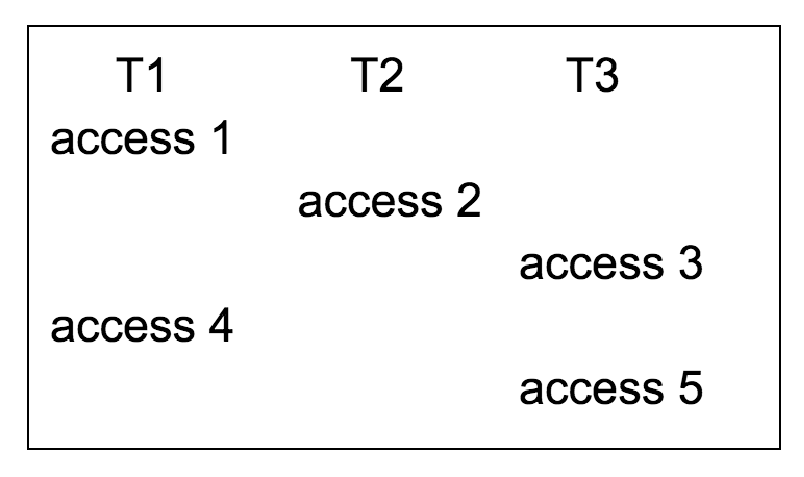
\epsfig{file=images/thread_accesses.eps, width=2in,}
\caption{Accesses to the same memory location from threads}
\end{figure}


Now that we have the instructions to form the window, we modified ThreadSanitizer to get information on the size of the window. To do that, we made ThreadSanitizer print the current timestamp in nanosecond scale with each access. Simply, the size of a window will be time difference between the beginning and the end of a window. To anticipate possible window size, we need to detect certain operations which might take long time under some condition. e.g. memory allocations, file operations, synchronization operations. Threadsanitizer already intercepts these operations. (refer to Appendix) For this project, we made ThreadSanitizer to print the size of allocated memory for each access so that we can compare the value at the beginning of a window to the value at the end. Similarly, we can do the same thing for file operations and synchronization operations as well.

After we get information of accesses, we do post-processing. The biggest reason is that threadsanitizer prints out the race reports as soon as it detects, so reordering should be done either at the end of threadsanitizer or at a different post-processor after the program is terminated. We found that modifying threadsanitizer further would not be productive. ThreadSanitizer imposes several restrictions that complicates development, for example, it has it's own memory allocation mechanism only allowed for predefined data types and cannot use the standard library. 

\subsection{Post-processing}
In the post processing, we form the vulnerability windows and order them. To form a window, post processor keeps all the access for each racy location, and make a window between accesses of the same thread. Figure xxx shows the data structure of post processor. While parsing the result from threadsanitizer, for each access, post processor stores information such as thread id, timestamp, memory access per location. In figure xxx, address 0xabcd has four different accesses. A window is formed whenever there are more than one accesses from the same thread. For the address 0xabcd, thread 1 forms a window, and it's size is 10ms which is determined by the time difference. Once the post processor parsed the whole result, then it reorders windows by size. Figure xxx is the typical output of post processor. It gives variable name, line number and thread id as well as window size, so with these information, developers can fix problems in the order of importance.

\begin{figure}
\centering
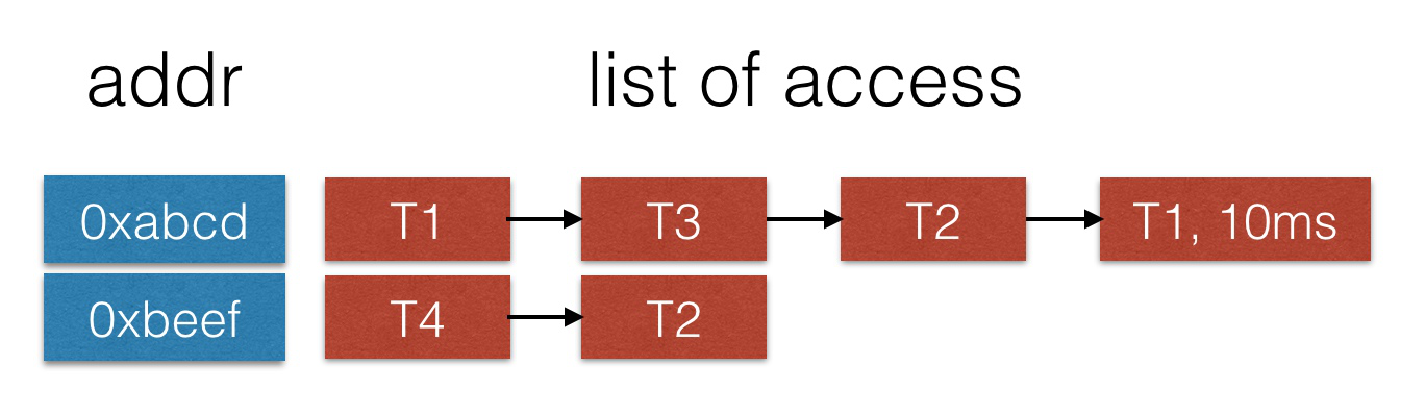
\epsfig{file=images/preprocessor.eps, width=\linewidth,}
\caption{Preprocessor data structure}
\end{figure}

\begin{figure}
\centering
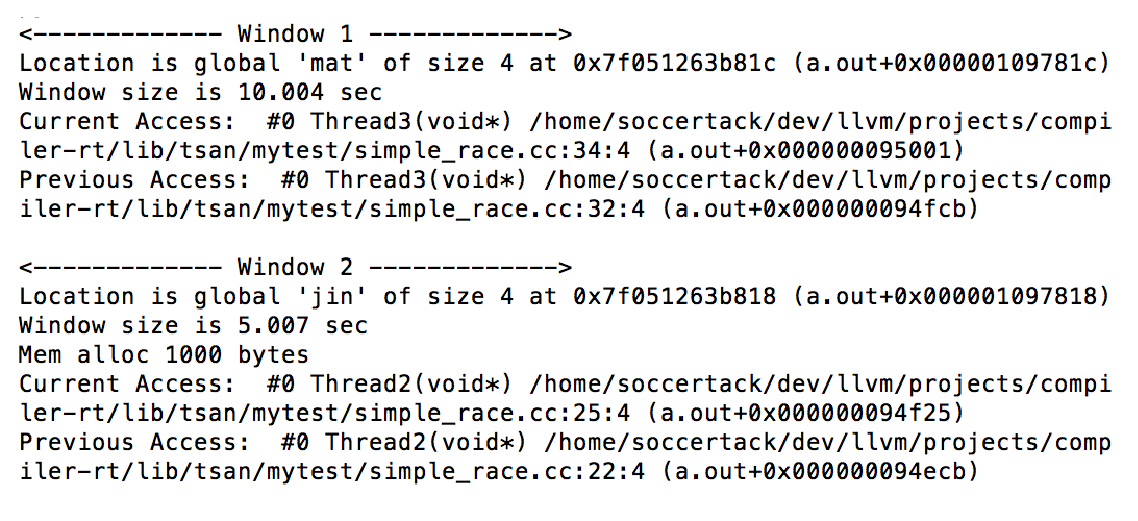
\epsfig{file=images/reorder.eps, width=\linewidth,}
\caption{Output of Preprocessor}
\end{figure}


\subsection{Data Flow Analysis}
Our data flow analysis implementation makes use of the data flow sanitizer distributed with LLVM. This sanitizer provides an interface that allow users to set, get and check the labels associated with variables, making it easy for developers to add data flow analysis to their application. Figure … shows the sanitizer interface. The Data Flow Sanitizer is actually still under development, but seems to be work for our sample programs. We chose to use it because it is the only data flow analysis implementation we know of, and implementing it on our own is out of the scope of this project.

Our implementation is divided into the instrumentation component and the runtime library. The runtime library contains the logic of how to test whether a memory location is dependent on the input or not.  The instrumentation component automatically insert calls to our runtime library inside the vulnerability window.

Our runtime library contains only two functions:
dfrtl\_check(addr, size)
Checks whether [addr, addr+size] is dependent on input. It prints the result to stderr for later processing.
dfrtl\_add\_input\_label(addr, size)
	Label [addr, addr+size] as input. Used to say what is considered input by the application.

	As we are only concerned about the code inside the vulnerability window, our instrumentation component needs as input the vulnerability window begin and end locations, which it receives from our post-process script. With these locations, the tool uses the debug information inserted by the compiler (with the '-g' flag) to find the associated instructions and then follows every possible path from the begin of window instruction until the end of the window instruction. In this pass, it collects the instruction that should had its operands checked for input dependence.

	Since our focus is to find input-controlled vulnerability window, we should check every instruction that could make the vulnerability window larger. In the limited time we had, we only implemented the instrumentation that checks whether a loop header condition is dependent on the input or not, giving us an idea of loops that can take longer because of input.

\begin{figure}
\centering
\epsfig{file=images/dflow.eps, width=\linewidth,}
\caption{DataFlowSanitizer Interface}
\end{figure}

\subsection{Tools Overview}

Figure … illustrates how the tools implemented work together. It starts by compiling the application with our modified ThreadSanitizer, which when run will output race reports. The reports are then processed by our post processing phase which forms the vulnerability window and pass it to the data flow tool, which will instrument, compile and run the application, outputting any cases where the input influences the vulnerability window. Our post processing phase is to back scene again to use this result and finally reorder the reports by size of the vulnerability window.

\begin{figure}
\centering
\epsfig{file=images/tooloverview.eps, width=\linewidth,}
\caption{Tool Overview}
\end{figure}


\section{Evaluation}
Typically, thetion of our tools was limited to just checking if it is working for simple toy examples. Even though we tried, we were not able to run big systems with ThreadSanitizer (i.e. Apache, Chromium, Firefox). We found it very hard to correctly modify the build process of these systems to use ThreadSanitizer, and for every single one of our tries we failed at some point. Nonetheless, we were able to use it for the examples we created, demonstrating that the problem was our limited knowledge of building very large systems. None of us have ever developed a system that required a complicated build process like the ones we tried.

\subsection{Static Alias Analysis}
Our static alias analysis attempt to form the vulnerability windows failed to achieve our expectations. When running alias analysis on an instruction which we knew always alias with the reported racy instruction, we received back the result “May alias”, which is the default result and does not give us any new information. When trying the memory dependence analysis, we received the result that the load instruction we were interested depended on a call to printf, which also is not very helpful since a printf function is read-only.

\subsection{Modified ThreadSanitizer and Postprocessing}
Our modification of threadsanitizer and post processor gives desired output like figure xxx successfully. 

\subsection{Data Flow Analysis}
Our data flow analysis implementation that looks for input-controlled loops inside the vulnerability window successfully outputs the dependence on the input when we tested with our toy examples. The dependence means that at least one of the loop conditions is dependent on the input. It does not tell us how big can it be made by changing the input, which would be ideal. We believe that by just reminding the developer that the loop is dependent on input is enough to help him/her better classify the bug.

Unfortunately, DataFlowSanitizer is still under development and does not yet support the whole standard library. For our toy examples, we had to add support for atoi to use our tool. We believe big systems would make use of many other ABI functions that are still not supported by the sanitizer, adding yet another problem to do a better evaluation of our project.


\section{Related Works}
This project was motivated by the paper Concurrency Attacks from Junfeng Yang et al. [Cite Junfeng], where many ideas came from. We are not aware of any other work that used the size of the vulnerability window as an indicative of the priority of a concurrency error. A similar work but with a different motivation have been previously done on measuring the probability of unserializable interleavings [Cite CTrigger]. In the CTrigger paper [Cite Ctrigger], they call a vulnerability window a 'gap' and they use profiling-run traces to identify those gaps, similar to how we got the time to execute the vulnerability window by modifying ThreadSanitizer to give us the time at the begin and end. We are not aware of any work about input-controlled vulnerability windows.

Our work focused on finding the vulnerability window associated with a data race report from ThreadSanitizer. Another approach would be to generalize to not only handle data races, but other concurrency errors too. An invariant-based atomicity bugs detector like AVIO [Cite AVIO] could be used instead of ThreadSanitizer for this goal. One benefit of using an invariant-based approach is that it already gives us the vulnerability window, since it is not predictive as the happens-before approach, saving us from the problems that we found when trying to find the vulnerability window. 

\section{Conclusion}
LLVM is helpful (LLVM IR and infrastructure), but its library are still not mature.




body of a paper is organized
into a hierarchical structure, with numbered or unnumbered
headings for sections, subsections, sub-subsections, and even
smaller sections.  The command \texttt{{\char'134}section} that
precedes this paragraph is part of such a
hierarchy.\footnote{This is the second footnote.  It
starts a series of three footnotes that add nothing
informational, but just give an idea of how footnotes work
and look. It is a wordy one, just so you see
how a longish one plays out.} \LaTeX\ handles the numbering
and placement of these headings for you, when you use
the appropriate heading commands around the titles
of the headings.  If you want a sub-subsection or
smaller part to be unnumbered in your output, simply append an
asterisk to the command name.  Examples of both
numbered and unnumbered headings will appear throughout the
balance of this sample document.

Because the entire article is contained in
the \textbf{document} environment, you can indicate the
start of a new paragraph with a blank line in your
input file; that is why this sentence forms a separate paragraph.

\subsection{Type Changes and {\subsecit Special} Characters}
We have already seen several typeface changes in this sample.  You
can indicate italicized words or phrases in your text with
the command \texttt{{\char'134}textit}; emboldening with the
command \texttt{{\char'134}textbf}
and typewriter-style (for instance, for computer code) with
\texttt{{\char'134}texttt}.  But remember, you do not
have to indicate typestyle changes when such changes are
part of the \textit{structural} elements of your
article; for instance, the heading of this subsection will
be in a sans serif\footnote{A third footnote, here.
Let's make this a rather short one to
see how it looks.} typeface, but that is handled by the
document class file. Take care with the use
of\footnote{A fourth, and last, footnote.}
the curly braces in typeface changes; they mark
the beginning and end of
the text that is to be in the different typeface.

You can use whatever symbols, accented characters, or
non-English characters you need anywhere in your document;
you can find a complete list of what is
available in the \textit{\LaTeX\
User's Guide}\cite{Lamport:LaTeX}.

\subsection{Math Equations}
You may want to display math equations in three distinct styles:
inline, numbered or non-numbered display.  Each of
the three are discussed in the next sections.

\subsubsection{Inline (In-text) Equations}
A formula that appears in the running text is called an
inline or in-text formula.  It is produced by the
\textbf{math} environment, which can be
invoked with the usual \texttt{{\char'134}begin. . .{\char'134}end}
construction or with the short form \texttt{\$. . .\$}. You
can use any of the symbols and structures,
from $\alpha$ to $\omega$, available in
\LaTeX\cite{Lamport:LaTeX}; this section will simply show a
few examples of in-text equations in context. Notice how
this equation: \begin{math}\lim_{n\rightarrow \infty}x=0\end{math},
set here in in-line math style, looks slightly different when
set in display style.  (See next section).

\subsubsection{Display Equations}
A numbered display equation -- one set off by vertical space
from the text and centered horizontally -- is produced
by the \textbf{equation} environment. An unnumbered display
equation is produced by the \textbf{displaymath} environment.

Again, in either environment, you can use any of the symbols
and structures available in \LaTeX; this section will just
give a couple of examples of display equations in context.
First, consider the equation, shown as an inline equation above:
\begin{equation}\lim_{n\rightarrow \infty}x=0\end{equation}
Notice how it is formatted somewhat differently in
the \textbf{displaymath}
environment.  Now, we'll enter an unnumbered equation:
\begin{displaymath}\sum_{i=0}^{\infty} x + 1\end{displaymath}
and follow it with another numbered equation:
\begin{equation}\sum_{i=0}^{\infty}x_i=\int_{0}^{\pi+2} f\end{equation}
just to demonstrate \LaTeX's able handling of numbering.

\subsection{Citations}
Citations to articles \cite{bowman:reasoning, clark:pct, braams:babel, herlihy:methodology},
conference
proceedings \cite{clark:pct} or books \cite{salas:calculus, Lamport:LaTeX} listed
in the Bibliography section of your
article will occur throughout the text of your article.
You should use BibTeX to automatically produce this bibliography;
you simply need to insert one of several citation commands with
a key of the item cited in the proper location in
the \texttt{.tex} file \cite{Lamport:LaTeX}.
The key is a short reference you invent to uniquely
identify each work; in this sample document, the key is
the first author's surname and a
word from the title.  This identifying key is included
with each item in the \texttt{.bib} file for your article.

The details of the construction of the \texttt{.bib} file
are beyond the scope of this sample document, but more
information can be found in the \textit{Author's Guide},
and exhaustive details in the \textit{\LaTeX\ User's
Guide}\cite{Lamport:LaTeX}.

This article shows only the plainest form
of the citation command, using \texttt{{\char'134}cite}.
This is what is stipulated in the SIGS style specifications.
No other citation format is endorsed.

\subsection{Tables}
Because tables cannot be split across pages, the best
placement for them is typically the top of the page
nearest their initial cite.  To
ensure this proper ``floating'' placement of tables, use the
environment \textbf{table} to enclose the table's contents and
the table caption.  The contents of the table itself must go
in the \textbf{tabular} environment, to
be aligned properly in rows and columns, with the desired
horizontal and vertical rules.  Again, detailed instructions
on \textbf{tabular} material
is found in the \textit{\LaTeX\ User's Guide}.

Immediately following this sentence is the point at which
Table 1 is included in the input file; compare the
placement of the table here with the table in the printed
dvi output of this document.

\begin{table}
\centering
\caption{Frequency of Special Characters}
\begin{tabular}{|c|c|l|} \hline
Non-English or Math&Frequency&Comments\\ \hline
\O & 1 in 1,000& For Swedish names\\ \hline
$\pi$ & 1 in 5& Common in math\\ \hline
\$ & 4 in 5 & Used in business\\ \hline
$\Psi^2_1$ & 1 in 40,000& Unexplained usage\\
\hline\end{tabular}
\end{table}

To set a wider table, which takes up the whole width of
the page's live area, use the environment
\textbf{table*} to enclose the table's contents and
the table caption.  As with a single-column table, this wide
table will ``float" to a location deemed more desirable.
Immediately following this sentence is the point at which
Table 2 is included in the input file; again, it is
instructive to compare the placement of the
table here with the table in the printed dvi
output of this document.


\begin{table*}
\centering
\caption{Some Typical Commands}
\begin{tabular}{|c|c|l|} \hline
Command&A Number&Comments\\ \hline
\texttt{{\char'134}alignauthor} & 100& Author alignment\\ \hline
\texttt{{\char'134}numberofauthors}& 200& Author enumeration\\ \hline
\texttt{{\char'134}table}& 300 & For tables\\ \hline
\texttt{{\char'134}table*}& 400& For wider tables\\ \hline\end{tabular}
\end{table*}
% end the environment with {table*}, NOTE not {table}!

\subsection{Figures}
Like tables, figures cannot be split across pages; the
best placement for them
is typically the top or the bottom of the page nearest
their initial cite.  To ensure this proper ``floating'' placement
of figures, use the environment
\textbf{figure} to enclose the figure and its caption.

This sample document contains examples of \textbf{.eps}
and \textbf{.ps} files to be displayable with \LaTeX.  More
details on each of these is found in the \textit{Author's Guide}.

\begin{figure}
\centering
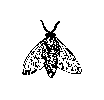
\epsfig{file=images/fly.eps}
\caption{A sample black and white graphic (.eps format).}
\end{figure}

\begin{figure}
\centering
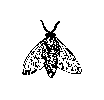
\epsfig{file=images/fly.eps, height=1in, width=1in}
\caption{A sample black and white graphic (.eps format)
that has been resized with the \texttt{epsfig} command.}
\end{figure}


As was the case with tables, you may want a figure
that spans two columns.  To do this, and still to
ensure proper ``floating'' placement of tables, use the environment
\textbf{figure*} to enclose the figure and its caption.

Note that either {\textbf{.ps}} or {\textbf{.eps}} formats are
used; use
the \texttt{{\char'134}epsfig} or \texttt{{\char'134}psfig}
commands as appropriate for the different file types.

\subsection{Theorem-like Constructs}
Other common constructs that may occur in your article are
the forms for logical constructs like theorems, axioms,
corollaries and proofs.  There are
two forms, one produced by the
command \texttt{{\char'134}newtheorem} and the
other by the command \texttt{{\char'134}newdef}; perhaps
the clearest and easiest way to distinguish them is
to compare the two in the output of this sample document:

This uses the \textbf{theorem} environment, created by
the\linebreak\texttt{{\char'134}newtheorem} command:
\newtheorem{theorem}{Theorem}
\begin{theorem}
Let $f$ be continuous on $[a,b]$.  If $G$ is
an antiderivative for $f$ on $[a,b]$, then
\begin{displaymath}\int^b_af(t)dt = G(b) - G(a).\end{displaymath}
\end{theorem}

The other uses the \textbf{definition} environment, created
by the \texttt{{\char'134}newdef} command:
\newdef{definition}{Definition}
\begin{definition}
If $z$ is irrational, then by $e^z$ we mean the
unique number which has
logarithm $z$: \begin{displaymath}{\log e^z = z}\end{displaymath}
\end{definition}

\begin{figure}
\centering
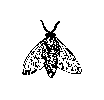
\epsfig{file=images/fly.eps, height=1in, width=1in,}
\caption{A sample black and white graphic (.ps format) that has
been resized with the \texttt{psfig} command.}
\end{figure}

Two lists of constructs that use one of these
forms is given in the
\textit{Author's  Guidelines}.

\begin{figure*}
\centering
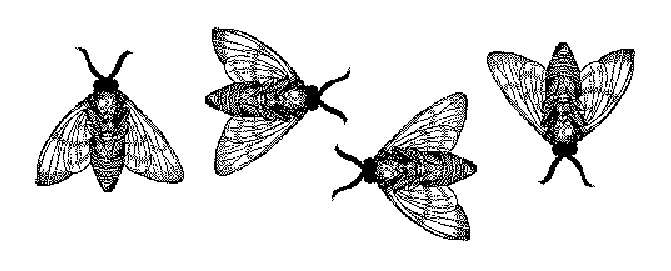
\epsfig{file=images/flies.eps}
\caption{A sample black and white graphic (.eps format)
that needs to span two columns of text.}
\end{figure*}
and don't forget to end the environment with
{figure*}, not {figure}!
 
There is one other similar construct environment, which is
already set up
for you; i.e. you must \textit{not} use
a \texttt{{\char'134}newdef} command to
create it: the \textbf{proof} environment.  Here
is a example of its use:
\begin{proof}
Suppose on the contrary there exists a real number $L$ such that
\begin{displaymath}
\lim_{x\rightarrow\infty} \frac{f(x)}{g(x)} = L.
\end{displaymath}
Then
\begin{displaymath}
l=\lim_{x\rightarrow c} f(x)
= \lim_{x\rightarrow c}
\left[ g{x} \cdot \frac{f(x)}{g(x)} \right ]
= \lim_{x\rightarrow c} g(x) \cdot \lim_{x\rightarrow c}
\frac{f(x)}{g(x)} = 0\cdot L = 0,
\end{displaymath}
which contradicts our assumption that $l\neq 0$.
\end{proof}

Complete rules about using these environments and using the
two different creation commands are in the
\textit{Author's Guide}; please consult it for more
detailed instructions.  If you need to use another construct,
not listed therein, which you want to have the same
formatting as the Theorem
or the Definition\cite{salas:calculus} shown above,
use the \texttt{{\char'134}newtheorem} or the
\texttt{{\char'134}newdef} command,
respectively, to create it.

\subsection*{A {\secit Caveat} for the \TeX\ Expert}
Because you have just been given permission to
use the \texttt{{\char'134}newdef} command to create a
new form, you might think you can
use \TeX's \texttt{{\char'134}def} to create a
new command: \textit{Please refrain from doing this!}
Remember that your \LaTeX\ source code is primarily intended
to create camera-ready copy, but may be converted
to other forms -- e.g. HTML. If you inadvertently omit
some or all of the \texttt{{\char'134}def}s recompilation will
be, to say the least, problematic.

\section{Conclusions}
This paragraph will end the body of this sample document.
Remember that you might still have Acknowledgments or
Appendices; brief samples of these
follow.  There is still the Bibliography to deal with; and
we will make a disclaimer about that here: with the exception
of the reference to the \LaTeX\ book, the citations in
this paper are to articles which have nothing to
do with the present subject and are used as
examples only.
%\end{document}  % This is where a 'short' article might terminate

%ACKNOWLEDGMENTS are optional
\section{Acknowledgments}
This section is optional; it is a location for you
to acknowledge grants, funding, editing assistance and
what have you.  In the present case, for example, the
authors would like to thank Gerald Murray of ACM for
his help in codifying this \textit{Author's Guide}
and the \textbf{.cls} and \textbf{.tex} files that it describes.

%
% The following two commands are all you need in the
% initial runs of your .tex file to
% produce the bibliography for the citations in your paper.
\bibliographystyle{abbrv}
\bibliography{report}  % report.bib is the name of the Bibliography in this case
% You must have a proper ".bib" file
%  and remember to run:
% latex bibtex latex latex
% to resolve all references
%
% ACM needs 'a single self-contained file'!
%
%APPENDICES are optional
%\balancecolumns
\appendix
%Appendix A
\section{Headings in Appendices}
The rules about hierarchical headings discussed above for
the body of the article are different in the appendices.
In the \textbf{appendix} environment, the command
\textbf{section} is used to
indicate the start of each Appendix, with alphabetic order
designation (i.e. the first is A, the second B, etc.) and
a title (if you include one).  So, if you need
hierarchical structure
\textit{within} an Appendix, start with \textbf{subsection} as the
highest level. Here is an outline of the body of this
document in Appendix-appropriate form:
\subsection{Introduction}
\subsection{The Body of the Paper}
\subsubsection{Type Changes and  Special Characters}
\subsubsection{Math Equations}
\paragraph{Inline (In-text) Equations}
\paragraph{Display Equations}
\subsubsection{Citations}
\subsubsection{Tables}
\subsubsection{Figures}
\subsubsection{Theorem-like Constructs}
\subsubsection*{A Caveat for the \TeX\ Expert}
\subsection{Conclusions}
\subsection{Acknowledgments}
\subsection{Additional Authors}
This section is inserted by \LaTeX; you do not insert it.
You just add the names and information in the
\texttt{{\char'134}additionalauthors} command at the start
of the document.
\subsection{References}
Generated by bibtex from your ~.bib file.  Run latex,
then bibtex, then latex twice (to resolve references)
to create the ~.bbl file.  Insert that ~.bbl file into
the .tex source file and comment out
the command \texttt{{\char'134}thebibliography}.
% This next section command marks the start of
% Appendix B, and does not continue the present hierarchy
\section{More Help for the Hardy}
The acm\_proc\_article-sp document class file itself is chock-full of succinct
and helpful comments.  If you consider yourself a moderately
experienced to expert user of \LaTeX, you may find reading
it useful but please remember not to change it.
\balancecolumns
% That's all folks!
\end{document}
